\documentclass[a4paper]{report}
\usepackage{apacite}
\usepackage{graphicx}
\usepackage{algorithm}
\usepackage{algcompatible}
\usepackage[section]{placeins}
\graphicspath{{Images/}}
\setlength\parindent{0pt}

\makeatletter
\AtBeginDocument{%
	\expandafter\renewcommand\expandafter\subsection\expandafter{%
		\expandafter\@fb@secFB\subsection
	}%
}
\makeatother

\begin{document}
	%------------------------Cover-------------------------------------------------------------
	\begin{titlepage} 
		\newcommand{\HRule}{\rule{\linewidth}{0.5mm}}
		
		\center 
		
		\textsc{\large Project 1.1 - Block 3}\\[0.5cm] 
		
		\HRule\\[0.4cm]
		
		{\huge\bfseries Compute chromatic numbers}\\[0.4cm] 
		
		\HRule\\[1.5cm]
		
		\textsc{\large Group 10}\\[0.5cm]

		\begin{minipage}{0.6\textwidth}
			\begin{flushleft}
				Tu Anh Dinh\\Michal Jarski\\Vaishnavi Velaga
			\end{flushleft}
		\end{minipage}
		~
		\begin{minipage}{0.3\textwidth}
			\begin{flushleft}
				Rudy Wessels\\Oskar Wielgos\\
			\end{flushleft}
		\end{minipage}
		
		\vspace{2cm}
		
		Submited: Wednesday January 23, 2019
		
		
	\end{titlepage}
	
	
	
	
	
	%-------------------Title page-----------------------------------------------------------
	\begin{titlepage} 
		\newcommand{\HRule}{\rule{\linewidth}{0.5mm}} 
		
		\center
		
		\textsc{\LARGE Maastricht University}\\[1.5cm]
		
		\textsc{\Large Department of Data Science and Knowledge Engineering}\\[0.5cm] 
		
		\textsc{\large Project 1.1 - Block 3}\\[0.5cm] 
		
		\HRule\\[0.4cm]
		
		{\huge\bfseries Compute chromatic numbers}\\[0.4cm] 
		
		\HRule\\[1.5cm]
		
		\textsc{\large Group 10}\\[0.5cm]
		
		\begin{minipage}{0.6\textwidth}
			\begin{flushleft}
				Tu Anh Dinh\\Michal Jarski\\Vaishnavi Velaga
			\end{flushleft}
		\end{minipage}
		~
		\begin{minipage}{0.3\textwidth}
			\begin{flushleft}
				Rudy Wessels\\Oskar Wielgos\\
			\end{flushleft}
		\end{minipage}
	
		 \vspace{1cm}
		Submited: Wednesday January 23, 2019
		\vspace{3cm}
		\begin{flushleft}
			Project coordinator: Prof. Jan Paredis
		\end{flushleft}
		
	\end{titlepage}
	
	%-----------------------------------------------------------------------------
	\chapter*{Preface}
	\pagenumbering{gobble}

	\addcontentsline{toc}{chapter}{Preface}
	This report is a part of the outcomes of our work for project 1.3: Graph Coloring. It can be used as a guideline to partially solve the non-deterministic polynomial-time hard problem of finding the chromatic number of a graph.
	
	
	%-----------------------------------------------------------------------------
	\chapter*{Summary}
	\addcontentsline{toc}{chapter}{Summary}
	This project gives an answer for the question of finding the smallest range of the chromatic number of a graph. The methods used are graph decomposition, greedy algorithm, identifying special cases of graphs, brute-force algorithm and genetic algorithm. This approach gives decent results on small graphs and graphs with special structures. However, the results are unpredictable for large arbitrary graphs.
	
	%-----------------------------------------------------------------------------
	\tableofcontents
	
%	\chapter*{Abbreviations and symbols}
%	\addcontentsline{toc}{chapter}{List of abbreviations and symbols}

	
	%-----------------------------------------------------------------------------
	\chapter{Introduction}
	\pagenumbering{arabic}
	
	A graph is a set of vertices connected by edges. In this project, the input graphs are undirected graph, where the edges have no orientation. In addition, a vertex must not connected to itself and the number of edges between two vertices must not exceed 1. \\
	
	Graph coloring is coloring the vertices of a graph such that no two adjacent vertices share the same color. Graph coloring is one of the important topic of graph theory and is used in real time applications of computer science and it is used in various research areas of computer science such as data mining, networking etc.\\
	
	The smallest number of colors used in graph coloring is called the chromatic number. A lower bound of a graph is a number that is less than or equal to the chromtic number, while an upper bound is a number that is greater than or equal to the chromtic number. The purpose of this project is to find the closest upper bound, lower bound and, if possible, the chromatic number of a graph.\\
	
	The rest of the report is divided as follows. Chapter 2 is about the methods used to compute the upper bound, lower bound and the chromatic number of a graph. Different algorithms are used: graph decomposition, greedy algorithm, identifying special cases of graphs, brute-force algorithm and genetic algorithm. Chapters 3,4 and 5 are about experiments and their results. In the last chapter, the whole project will be concluded.
	
	\chapter{Methods}
	This chapter describes the methods used for finding the lower bound, upper bound and if possible, the chromatic number of a graph. 
	\section{Overview}
	Given the limitation on execution time (2 minutes for each graph in the tournament), methods that give out results fast are executed first. Algorithm \ref{alg:overview} describes the general work flow.\\
	\begin{algorithm}
		\caption{General work flow}
		\label{alg:overview}
		\begin{algorithmic}[1]
			\REQUIRE a graph
			\STATE upperbound = greedyUpperbound(graph)
			\STATE components = decompose(graph)
			\FORALL{components} 
				
				\STATE//Check all special cases
				\IF{component has no vertex} 
					\STATE chromaticNumber of component = 0
					\STATE Go to the next component
				\ENDIF
				\IF{component has no edge} 
				\STATE chromaticNumber of component = 1
				\STATE Go to the next component
				\ENDIF
				\IF{component is bipartite} 
				\STATE chromaticNumber of component = 2
				\STATE Go to the next component
				\ENDIF
				\IF{component is odd cycle} 
				\STATE chromaticNumber of component = 3
				\STATE Go to the next component
				\ENDIF
				\IF{component is complete graph} 
				\STATE chromaticNumber of component = number of vertices
				\STATE Go to the next component
				\ENDIF
				
				\STATE subUpperbound =  greedyUpperbound(component)
				\STATE subLowerbound =  greedyLowerbound(component)
				
				\STATE newSubLowerbound = 3
				\STATE Update subLowerBound if needed
				\IF{subUpperbound = subLowerbound} 
				\STATE chromaticNumber of component = subUpperbound
				\STATE Go to the next component
				\ENDIF
				
				\STATE//Run brute-force
				\IF{number of vertices $<=$ 20} 
				\STATE chromaticNumber of component = BruteForce(component)
				\ENDIF 
			\ENDFOR

			\algstore{myalg}
			\end{algorithmic}
		\end{algorithm}

		\begin{algorithm}                     
			\begin{algorithmic} [1]     
			\algrestore{myalg}

			\STATE newUpperbound = max(subUpperbounds)
			
			\IF{newUpperbound $<$ upperbound} 
			\STATE //Update upper bound
			\STATE upperbound = newUpperbound 
			\ENDIF
			
			\STATE lowerbound = max(subLowerbounds)
			
			\IF{has found all chromatic numbers of components} 
			\STATE chromatic number = max(chromatic numbers of components)
			\ELSE
			\STATE lowerbound = max(chromatic numbers of components)
			\ENDIF
			
			\STATE geneticAlgorithm(graph)
		\end{algorithmic}
	\end{algorithm}
	First, a greedy algorithm is run on the given graph to calculate the upper bound (line 1). Then, the given graph is decomposed to connected components. Each component is checked to see if it is one of the special cases where the chromatic number can be concluded immediately (line 5 - 24). The special cases are listed below: 
	\begin{itemize}
		\item No-vertex graph: chromatic number is 0
		\item No-edge graph: chromatic number is 1
		\item Bipartite graph: chromatic number is 2
		\item Odd cycle: chromatic number is 3
		\item Complete graph: chromatic number is the number of vertices
	\end{itemize}
	Next, a lower bound and an upper bound are computed by greedy algorithms (line 25 and 26). The reason for running greedy algorithm for upper bound on both the original graph and its components is that the result upper bounds are sometimes different, so we run both cases to get the better upper bound.  However, the greedy algorithm for lower bound normally gives the same results for both cases, so it is run only on the components
	In line 27, if a component is none of the special cases then a lower bound of the component is 3, since the first three cases have covered all graphs where the chromatic number is below 3. It is then compared to the previous lower bound computed in line 26 to update the lower bound if needed. Next, if the lower bound and upper bound are equal, then the chromatic number can be concluded(line 29 - 32). \\
	If the chromatic number of a component still cannot be calculated then a brute-force algorithm is used (line 34 - 36). However, only components with number of vertices below 20 are proccessed with the brute-force algorithm, since the brute-force algorithm normally takes longer than 2 minutes to execute on bigger graphs. Without the time-restriction of 2 minutes, the more time we have, the higher the threshold for brute-force can be (about 30 to 40).\\
	
	After proccessing on the components, the upper bound, the lower bound and possibly the chromatic number of the original graph can be concluded. The biggest upper bound among the components is the upper bound of the original graph (line 38). This new upper bound is then compared to the previously computed upper bound in line 1 to output the better one. Similarily, the biggest lower bound among the components is a lower bound of the original graph (line 43). \\
	If the chromatic numbers of all components have been found, then the chromatic number of the original graph is the biggest chromatic number among the components (line 44-45). If it is not the case, then the biggest chromatic number found on the components is another lower bound for the original graph (line 47).\\
	Finally, in line 49, genetic algorithm is used to bring the upper bound closer to the chromatic number. Genetic algorithm is run last because there is no guarantee on its execution time.\\
	
	The algorithm for each method is described in the next sections of this chapter.
	

		\section{Graph decomposition}
		One graph can contain multiple disconnected parts, which can be considered as independent subgraphs (Figure \ref{fig:decompose}). Decomposition means seperating the graph into fully connected components. Decomposing the graph will allow other methods to work on smaller graphs. Algorithm \ref{alg:decompose} describes the method for decomposing a graph into components.\\
		
		\begin{figure}[h]
			\centering
			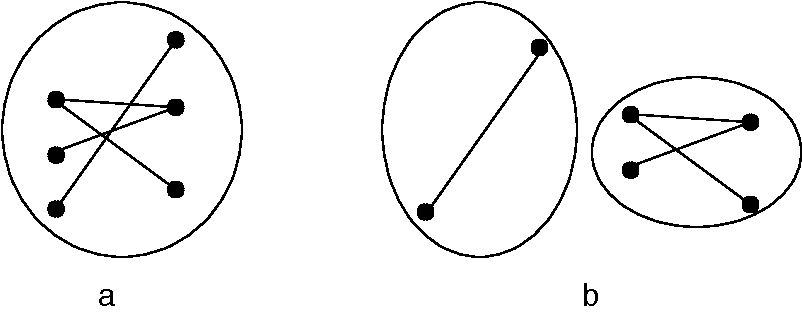
\includegraphics[width=50mm,scale=0.5]{figures/DecomposedGraph.pdf}
			\caption{A graph (a) before decomposed and (b) after decomposed}
			\label{fig:decompose}
		\end{figure}
	
		\begin{algorithm}
			\caption{Decomposing a graph}
			\label{alg:decompose}
			\begin{algorithmic}[1]
				\REQUIRE a graph
				\STATE Create listOfVertices 
				\STATE listOfVertices.add(all vertices in the graph)
				\WHILE{listOfVertices is not empty}
				\STATE Create a new component
				\STATE Create a new uncheckedList
				\STATE component.add(firstVertex in listOfVertices )
				\STATE uncheckedList.add(firstVertex in listOfVertices)
				\STATE listOfVertices.remove(first element)
				\WHILE{uncheckedList is not empty} 
				\STATE checkingVertex = first vertex in the uncheckedList
				\FORALL{neighbors of checkingVertex} 
				\IF{neighbor is not in component} 
				\STATE uncheckedList.add(neighbor)
				\STATE component.add(neighbor)
				\ENDIF
				\STATE listOfVertices.remove(neighbor)
				\ENDFOR
				\STATE Remove checkingVertex from uncheckedList
				\ENDWHILE
				\STATE Convert component to standard form
				\STATE components.add(component)
				\ENDWHILE
				\STATE \textbf{return} components
				
			\end{algorithmic}
		\end{algorithm}
		The algorithm is based on breadth-first search. A unchecked-list stores the vertices whose neighbors are not yet added to the current expanding component. In line 6 and 7 the first vertex is added to a component and the unchecked list. Then all the neighbors of the vertex are added to the component and the unchecked list, and the first vertex of the unchecked list is removed (line 9 - 19). To avoid loops, only vertices not in the component are added. The same is done for all vertices in the unchecked list, until the list is empty. The process is repeated until all vertices in the original graph are classified into components.\\
		Note that the vertices of the input graphs for this project are represented by successive numbers. All algorithms are implemented based on this data structure. Therefore, after classifying the vertices into components, each component is then converted to the standard form, where the indexes of vertices are successive numbers (line 20).
		
		\section{Greedy algorithm for upper bound}
		Greedy algorithm for upper bound provides an efficient way of coloring a graph. However, it does not guarantee that the coloring is optimal. Therefore, it can be used to calculate a upper bound. Algorithm \ref{alg:greedy} \cite{jensen2011graph} describes this method.\\
		\begin{algorithm}
			\caption{Greedy algorithm for upper bound}
			\label{alg:greedy}
			\begin{algorithmic}[1]
				\REQUIRE a graph
				\STATE Sort vertices in non-increasing order of constraints (the number of neighbors)
				\STATE Create availableColors list
				\FORALL{vertices}
					\FORALL{colors in availableColors}
					\IF{color is valid for vertex}
					\STATE Assign the color for the vertex
					\STATE break
					\ENDIF
					\ENDFOR
					\IF{The vertex is still not colored}
					\STATE Create a new color
					\STATE Assign the new color for the vertex
					\STATE Add the new color to availableColors list
					\ENDIF
				\ENDFOR
				\STATE \textbf{return} size of availableColors list
			\end{algorithmic}
		\end{algorithm}
		First, the vertices are sorted based on their constraints (line 1). The constraint of a vertex is the number of other vertices connected to that vertex. The vertex with more neighbors will be colored first.\\
		A list is used to store available colors. When coloring a vertex, the available colors is reused as much as possible (line 4-9). If none of the available colors is valid to color that vertex, then a new color is generated and added to the available list (line 10-14). When the graph is fully colored, the number of colors in the available list is returned.\\
		
		\section{Greedy algorithm for lower bound}
		A greedy algorithm is used to find several cliques in a graph and returns the size of the biggest clique found \cite{steven2008algorithm}. The biggest size is then return as a lower bound. However, it does not guarantee to find the maximum clique. \\
		The algorithm works as follows. To form a clique, an initial vertex is added to the clique. Then, for every other vertex, we add it to the clique if it is connected to all vertices currently in the clique. The same proccess is repeated to find multiple cliques, where every vertex in the original graph is used as the initial vertex for a clique. 
		
		\section{Special cases}
			\subsection{Bipartite}
			A bipartite graph is a graph which its vertices can be separated into two sets such that there is no connection between any pair of vertices of the same set.\\
			The chromatic number of a bipartite graph is 2. Algorithm \ref{alg:bipartite} \cite{sedgewick2003} describes the steps to test weather a graph is bipartite, using breadth-first search. \\
			
			\begin{figure}[h]
				\centering
				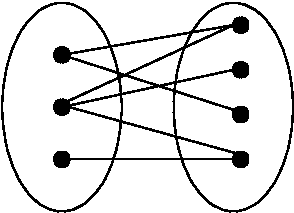
\includegraphics[width=50mm,scale=0.5]{figures/bipartite.pdf}
				\caption{An example of bipartite graphs}
				\label{fig:bipartite}
			\end{figure}
			
			\begin{algorithm}
				\caption{Bipartite testing}
				\label{alg:bipartite}
			
				\begin{algorithmic}[1]
					\REQUIRE a graph
					\STATE Create unchecked list
					\STATE unchecked.add(first vertex)
					\STATE Assign one color to the first vertex
					\WHILE{The graph is not fully colored}
					\WHILE{unchecked list is not empty}
					\STATE checkingVertex = unchecked.getFirstElement()
					\STATE unchecked.removeFistElement
					\FORALL{neighbors of checkingVertex}
					\IF{neibor not yet colored}
					\STATE Assign the opposite color of checkingVertex's color to neighbor
					\STATE unchecked.add(neighbor)
					\ELSIF{neighbor has invalid color}
					\STATE \textbf{return} false
					\ENDIF
					\ENDFOR
					\ENDWHILE
					\ENDWHILE
					\STATE \textbf{return} true
				\end{algorithmic}
			\end{algorithm}
			 Two colors are used to color the graph. A unchecked list stores the vertices whose neighbors are not yet considered. First, one color is assigned to the first vertex and the first vertex is added to the unchecked list (line 2-3). Then, all its neighbors are considered and the vertex itself is removed from the unchecked list. For each neighbor, if the neighbor has not been colored then it is assigned with the oposite color (line 10). If the neighbor has been colored, then we check if it is a valid coloring. If the coloring is invalid, the graph is not bipartite (line 12-13). The same is done for all elements in the unchecked list, until the list is empty. The process is repeated until all vertices in the graph are colored. If the graph is successfully colored, then it is bipartite.
			\subsection{Odd cycle}
			An odd cycle is a cycle with an odd number of edges and vertices (Figure \ref{fig:oddcycle}). The chromatic number of an odd cycle graph is 3. \\
			
			\begin{figure}[h]
				\centering
				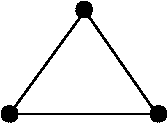
\includegraphics[width=50mm,scale=0.5]{figures/cycle.pdf}
				\caption{An example of odd cycle graphs}
				\label{fig:oddcycle}
			\end{figure}
		
			The method for testing if a graph is an odd cycle checks for three condition:
			\begin{itemize}
				\item The number of vertices is equal to the number of edges
				\item Every vertex has two neighbors
				\item The number of vertices is odd
			\end{itemize}
			A graph is an odd cycle graph if and only if all three conditions are satisfied.
			
			\subsection{Complete graph}
			A complete graph (Figure \ref{fig:complete}) is a graph where every vertex is connected to all other vertices. The chromatic number of a complete graph is the number of vertices. The method checks weather a graph has the above conditions to determine if it is a complete graph.
			\begin{figure}[h]
				\centering
				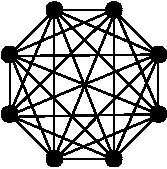
\includegraphics[width=50mm,scale=0.5]{figures/complete.pdf}
				\caption{An example of complete graphs}
				\label{fig:complete}
			\end{figure}
			
		\section{Brute-force algorithm}
		The brute-force algorithm simply generates every possible coloring and checks if it's a valid one. In case the coloring is valid, the algorithm terminates with a possibilty of returning an array of colors assigned to each node and the chromatic number. In order to check the validity of coloring, it utilizes isValid algorithm, that iterates through the array representing nodes' colors and searches for a conflict (two adjacent/connected nodes having assigned the same color). If found, false is being returned instantly, meaning certain coloring is not a valid one.\\
		
		Brute-force is based on raw computetional power, thus making it heavily dependent on the hardware that runs it. Finding the chromatic number is GUARANTEED sooner or later. However in reality, its use is limited to graphs not bigger than 20 nodes, and even then, depending yet on how the vertices are being connected.\\
		
		Algorithms calculating lower bound or applying pruning, might futher optimize it, reducing the time needed to find the chromatic number. \\
		
		Implementing a greedy-type brute-force could also bring significant improvements on effectivness and execution time, but on the other hand, causing a risk of omitting the right coloring and eventually not finding the chromatic number, but only its approximation.	
			
		\section{Genetic algorithm}
%			\subsection{Fitness function}
%			\subsection{Selection method}
%			\subsection{Crossover}
%			\subsection{Mutation}
		The genetic algorithm is an algorithm for calculating the upper bound together with working its way down to finding lower and better upper bounds for a particular graph. It starts with creating a population of individuals each containing a randomly colored version of the selected graph. The size of this population can be set to any number preferred. Once the population is created it assigns a fitness (which is a real number between 0 and 1) to each individual based on the number of incorrect edges. Following up the individuals are sorted by fitness from high to low (1$>$0), at which it becomes clear what part of the population has the highest correctness of coloring.\\
		
		After the individuals are sorted the selection method picks out the “parents” for the next generation through an elitist approach. These parents are utilized for the crossover method creating combinations of two of the parents until there are enough new individuals for the next generation with equal size to the previous one. Afterward, the mutation method, depending on the extent of the mutation rate, will mutate some individuals’ coloring of the graph to achieve possibly better results. By results is meant, individuals with higher fitness.
\\
		
		Lastly, this process runs over several generations/populations through a loop till the algorithm finds an individual with fitness “1” (no incorrect edges). When this is the case, the new upper bound will be printed in the command prompt based on how many colors were used to achieve this solution. Following up the entire process starts over with one less color, so that the upper bound will be lower after each successful finding.
		
		
		
	\chapter{Experiments}
	The experiment is set up to run on the given 20 graphs from phase 3 of the project. Each graph is exploited to see its properties:
	\begin{itemize}
		\item The number of vertices (or the size of the graph)
		\item The number of connected components
		\item The size of each component
		\item The number of components that are special cases
		\item The biggest clique found
	\end{itemize}

	\chapter{Results}

		\begin{table} [h!]
		\begin{center}
			\begin{tabular}{| c | c | c | c |c|}
				\hline
				Graph no. & Upper bound & Lower bound & Chromatic number & Gap \\
				\hline
				1 & 3 & $-$ & 3 & 0\\
				\hline
				2 & 5 & 3 & $-$ & 2\\
				\hline
				3 & 8 & 6 & $-$ & 2\\
				\hline
				4 & 7 & 4 & $-$ & 3\\
				\hline
				5 & 2 & $-$ & 2 & 0\\
				\hline
				6 & 3 & $-$ & 3 & 0\\
				\hline
				7 & 12 & 8 & $-$ & 4\\
				\hline
				8 & 98 & $-$ & 98 & 0\\
				\hline
				9 & 6 & 3 & $-$ & 3\\
				\hline
				10 & 3 & $-$ & 3 & 0\\
				\hline
				11 & 15 & 15 & 15 & 0\\
				\hline
				12 & 2 & $-$ & 2 & 0\\
				\hline
				13 & 14 & 9 & $-$ & 5\\
				\hline
				14 & 5 & 3 & $-$ & 2\\
				\hline
				15 & 10 & 5 & $-$ & 5\\
				\hline
				16 & 4 & 3 & $-$ & 1\\
				\hline
				17 & 8 & $-$ & 8 & 0\\
				\hline
				18 & 11 & 10 & $-$ & 1\\
				\hline
				19 & 11 & 11 & 11 & 0\\
				\hline
				20 & 9 & 8 & $-$ & 1\\
				\hline
			\end{tabular}
		\end{center}
		\caption{Results on the given 20 graphs from phase 3. The column "Gap" represents the differences between upper bounds and lower bounds}
		\label{tab:result}
	\end{table}
	
	\begin{table} [h!]
		\begin{center}
			\begin{tabular}{| c | c | c | c |c|c|c|}
				\hline
				Graph no. & Size & \shortstack{Number of \\ components}& Components' sizes & Special cases&\shortstack{Biggest clique\\ found}& Gap \\
				\hline
				1 & 212 & 1 & 212 &0&3& 0\\
				\hline
				2 & 456 & 8 & 448, 2, 1 (6 times) &7&3& 2\\
				\hline
				3 & 218 & 2 & 212, 6 &1&3& 2\\
				\hline
				4 & 107 & 1 & 107 &0&4& 3\\
				\hline
				5 & 4007 & 1 & 4007 &1&$-$& 0\\
				\hline
				6 & 529 & 260 & 8, 5, 2 (258 times) &260&$-$& 0\\
				\hline
				7 & 43 & 1 & 43 &0&8& 4\\
				\hline
				8 & 107 & 1 & 107 &0&98& 0\\
				\hline
				9 & 206 & 1 & 206 &0&3& 3\\
				\hline
				10 & 166 & 1 & 166 &0&2& 0\\
				\hline
				11 & 164 & 1 & 164 &0&15& 0\\
				\hline
				12 & 744 & 1 & 744 &1&$-$& 0\\
				\hline
				13 & 85 & 1 & 85 &0&9& 5\\
				\hline
				14 & 907 & 1 & 907 &0&3& 2\\
				\hline
				15 & 215 & 1 & 215 &0&5& 5\\
				\hline
				16 & 164 & 1 & 164 &0&2& 1\\
				\hline
				17 & 106 & 12 & 92, 2, 3, 1 (9 times) &11&8& 0\\
				\hline
				18 & 131 & 5 & 26 (2 times), 25 (2 times), 29 &0&10& 1\\
				\hline
				19 & 143 & 1 & 143 &0&11& 0\\
				\hline
				20 & 387 & 1 & 387 &0&8& 1\\
				\hline
			\end{tabular}
		\end{center}
		\caption{Properties of the given 20 graphs from phase 3, along with the gaps between upper bounds and lower bounds found}
		\label{tab:prop}
	\end{table}
	\chapter{Discussion}
	As can be seen from the results, our algorithms perform well to find the chromatic number on several types of graphs:
	\begin{itemize}
		\item For graphs that are special cases, the chromatic numbers can be found quickly, even if the graphs' sizes are large. For example, the sizes of graph 5 and graph 12 are 4007 and 744 respectively, but since they are bipartite graphs, their chromatic numbers were found in less than 1 minute.
		\item For graphs that are disconnected, the results are also good. For example, graph 2, 3, 6, and 17 can be decomposed into 8, 2, 260, 12 and 5 components respectively, so their ranges for chromatic numbers are small (less than or equal to 2).
		\item For graphs that have big clique sizes compared to the graphs' sizes, the gaps between the upper bounds and lower bounds found are small. For example, graph 8 has the size of 107 and the biggest clique size found is 98, so our algorithms can find its chromatic number.
	\end{itemize}
	On the other hand, the algorithms do not give as good results on certain graphs that do not have special structures. For example, graph 13 and 15 are fully connected, not special cases and their biggest clique sizes found are small compared to the graphs' sizes. Therefore, their ranges for chromatic number are higher (where the differences between upper bounds and lower bounds are both 5).
	
	\chapter{Conclusion}
	
	
	\bibliographystyle{apacite}
	\bibliography{references}
	
%	\appendix
%	\chapter*{Appendix}
%	\addcontentsline{toc}{chapter}{Appendix}
\end{document}